\chapter{実験結果}

%% 市街地でのシークエンスでの走行結果を書く
\section{実験結果}\label{sec:result}

\subsection{自己位置推定の精度}\label{sec:verify_localization}

\subsubsection{XYZ座標推定の精度}
メッシュ地図及び点群地図における自己位置推定において, 自己位置推定によって推定された位置とground truthとの間にどれほどの差があったかを割合で図\ref{fig:mesh_sequence00_XYZ}から図\ref{fig:point_sequence08_XYZ}にかけて示す. また, 実験においてGround truthの移動量からガウス分布に従う誤差を加えたオドメトリを用いて事前分布の更新を行った. このとき用いたオドメトリ, 「biased odometry」の位置とGround truthの位置との間にどれほどの差があったかも併せて図に示す.
\par 先行研究\cite{semantic_point_localization}については論文内では精度のいい自己位置推定の結果が示されていたが今回の実験においてはいずれのシークエンスでも自己位置推定が完全に破綻しており有効な結果は得られなかった. その一方で提案手法はいずれのシークエンスでも自己位置推定が破綻することなく安定した動作が見られた. しかしsequence05を除き, いずれのシークエンスでも1.5m以上2.0m以下の誤差が最頻値であったことから提案手法は今回の実験環境においては数cm単位での高い自己位置推定の精度を保証するものではない事が判明した. また, 時速30km以上での走行を行っているときは先行研究での手法と提案手法の両方で正確な自己位置推定ができなくなった. sequence05において自己位置推定がどの手法でも破綻したのはこのためであり, この原因については\ref{sec:considerarion}節で詳しく述べる.

\subsubsection{RPY方向推定の精度}
メッシュ地図及び点群地図における自己位置推定において, 自己位置推定によって推定された角度とground truthとの間にどれほどの差があったかを割合で図\ref{fig:mesh_sequence00_RPY}から図\ref{fig:point_sequence08_RPY}にかけて示す. \par 既存手法による角度推定ではsequence08等においてground truthと大きく異る値になることが頻繁に起こっていたが, 提案手法による角度推定においてはいずれのシークエンスでも誤差が概ね10度以下に収まるといった良好な結果が得られた.

\begin{figure}[htbp]
 \begin{minipage}{1.0\hsize}
  \begin{center}
   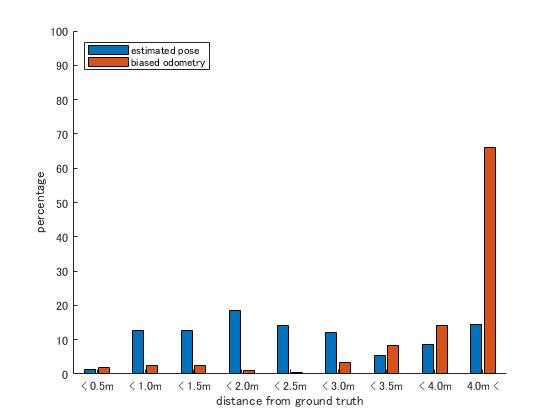
\includegraphics[width=110mm]{./picture/mesh_s0_xyz.jpg}
  \end{center}
  \caption{Sequence00における提案手法での自己位置推定精度}
  \label{fig:mesh_sequence00_XYZ}
 \end{minipage}
\end{figure}

\begin{figure}[htbp]
 \begin{minipage}{1.0\hsize}
  \begin{center}
   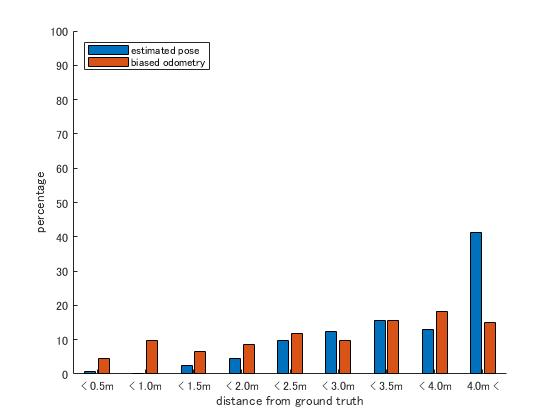
\includegraphics[width=110mm]{./picture/point_s0_xyz.jpg}
  \end{center}
  \caption{Sequence00における比較手法での自己位置推定精度}
  \label{fig:point_sequence00_XYZ}
 \end{minipage}
\end{figure}
 
\begin{figure}[htbp]
  \begin{minipage}{1.0\hsize}
  \begin{center}
   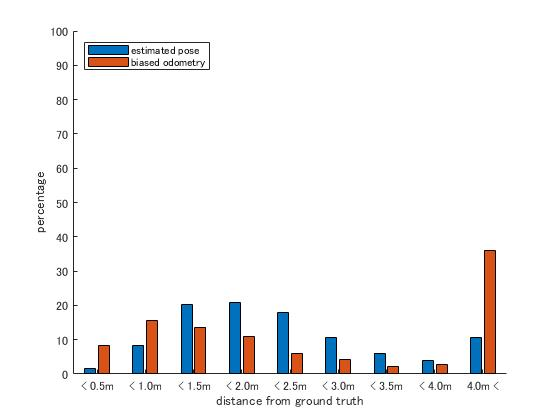
\includegraphics[width=110mm]{./picture/mesh_s2_xyz.jpg}
  \end{center}
  \caption{Sequence02における提案手法での自己位置推定精度}
  \label{fig:mesh_sequence02_XYZ}
 \end{minipage}
\end{figure}

\begin{figure}[htbp]
 \begin{minipage}{1.0\hsize}
  \begin{center}
   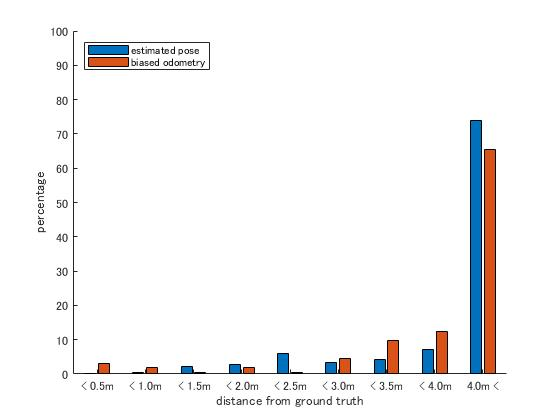
\includegraphics[width=110mm]{./picture/point_s2_xyz.jpg}
  \end{center}
  \caption{Sequence02における比較手法での自己位置推定精度}
  \label{fig:point_sequence02_XYZ}
 \end{minipage}
\end{figure}

\begin{figure}[htbp]
  \begin{minipage}{1.0\hsize}
  \begin{center}
   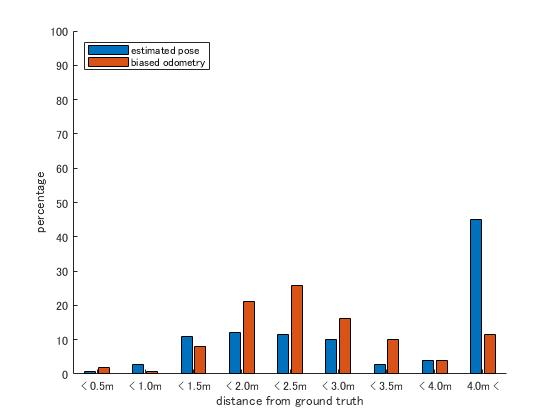
\includegraphics[width=110mm]{./picture/mesh_s5_xyz.jpg}
  \end{center}
  \caption{Sequence05における提案手法での自己位置推定精度}
  \label{fig:mesh_sequence05_XYZ}
 \end{minipage}
\end{figure}

\begin{figure}[htbp]
 \begin{minipage}{1.0\hsize}
  \begin{center}
   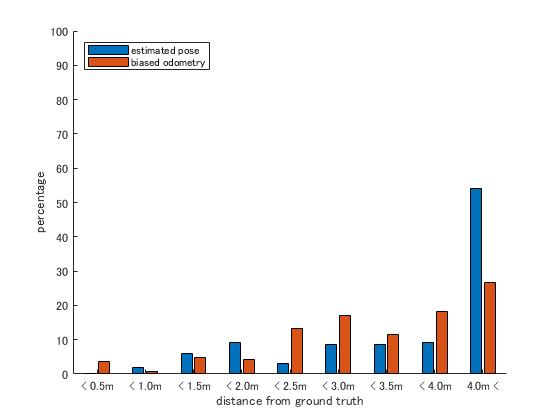
\includegraphics[width=110mm]{./picture/point_s5_xyz.jpg}
  \end{center}
  \caption{Sequence05における比較手法での自己位置推定精度}
  \label{fig:point_sequence05_XYZ}
 \end{minipage}
\end{figure}

\begin{figure}[htbp]
  \begin{minipage}{1.0\hsize}
  \begin{center}
   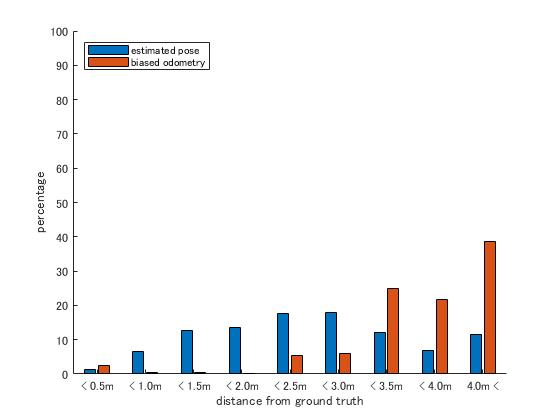
\includegraphics[width=110mm]{./picture/mesh_s8_xyz.jpg}
  \end{center}
  \caption{Sequence08における提案手法での自己位置推定精度}
  \label{fig:mesh_sequence08_XYZ}
 \end{minipage}
\end{figure}

\begin{figure}[htbp]
 \begin{minipage}{1.0\hsize}
  \begin{center}
   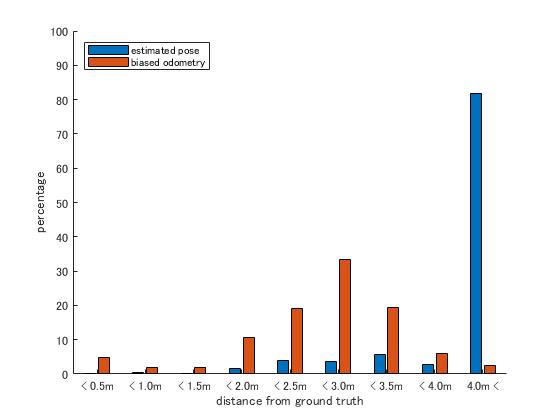
\includegraphics[width=110mm]{./picture/point_s8_xyz.jpg}
  \end{center}
  \caption{Sequence08における比較手法での自己位置推定精度}
  \label{fig:point_sequence08_XYZ}
 \end{minipage}
\end{figure}


\begin{figure}[htbp]
 \begin{minipage}{1.0\hsize}
  \begin{center}
   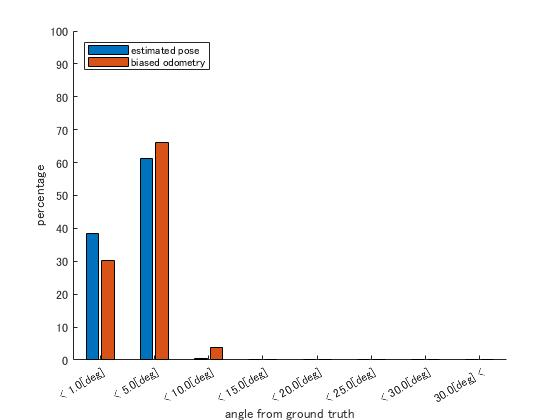
\includegraphics[width=110mm]{./picture/mesh_s0_rpy.jpg}
  \end{center}
  \caption{Sequence00における提案手法での角度推定精度}
  \label{fig:mesh_sequence00_RPY}
 \end{minipage}
\end{figure}

\begin{figure}[htbp]
 \begin{minipage}{1.0\hsize}
  \begin{center}
   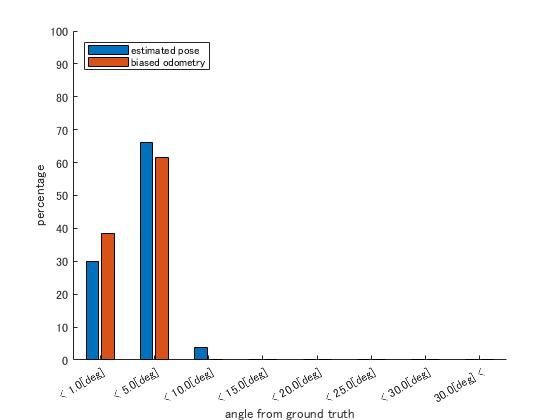
\includegraphics[width=110mm]{./picture/point_s0_rpy.jpg}
  \end{center}
  \caption{Sequence00における比較手法での角度推定精度}
  \label{fig:point_sequence00_RPY}
 \end{minipage}
\end{figure}
 
\begin{figure}[htbp]
  \begin{minipage}{1.0\hsize}
  \begin{center}
   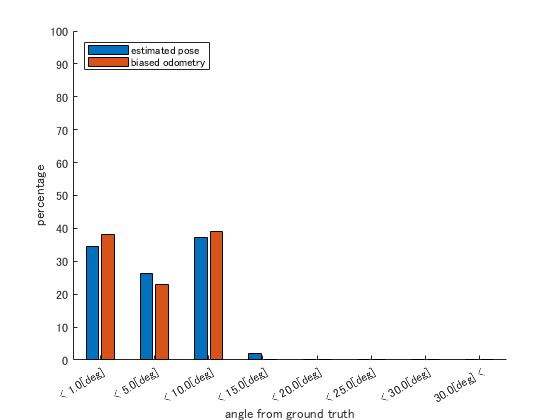
\includegraphics[width=110mm]{./picture/mesh_s2_rpy.jpg}
  \end{center}
  \caption{Sequence02における提案手法での角度推定精度}
  \label{fig:mesh_sequence02_RPY}
 \end{minipage}
\end{figure}

\begin{figure}[htbp]
 \begin{minipage}{1.0\hsize}
  \begin{center}
   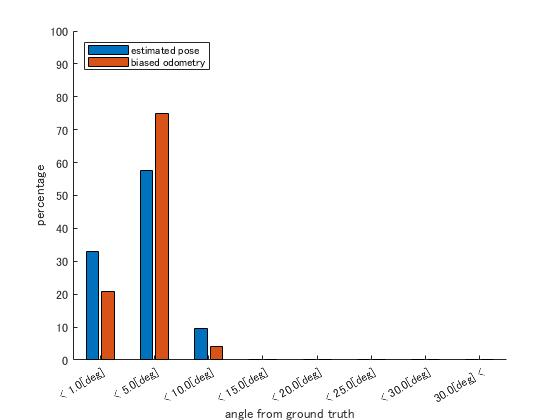
\includegraphics[width=110mm]{./picture/point_s2_rpy.jpg}
  \end{center}
  \caption{Sequence02における比較手法での角度推定精度}
  \label{fig:point_sequence02_RPY}
 \end{minipage}
\end{figure}

\begin{figure}[htbp]
  \begin{minipage}{1.0\hsize}
  \begin{center}
   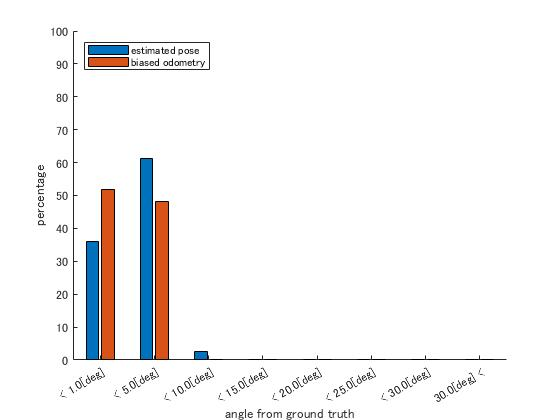
\includegraphics[width=110mm]{./picture/mesh_s5_rpy.jpg}
  \end{center}
  \caption{Sequence05における提案手法での角度推定精度}
  \label{fig:mesh_sequence05_RPY}
 \end{minipage}
\end{figure}

\begin{figure}[htbp]
 \begin{minipage}{1.0\hsize}
  \begin{center}
   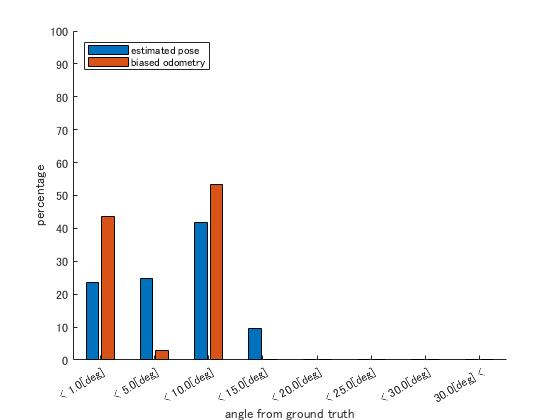
\includegraphics[width=110mm]{./picture/point_s5_rpy.jpg}
  \end{center}
  \caption{Sequence05における比較手法での角度推定精度}
  \label{fig:point_sequence05_RPY}
 \end{minipage}
\end{figure}

\begin{figure}[htbp]
  \begin{minipage}{1.0\hsize}
  \begin{center}
   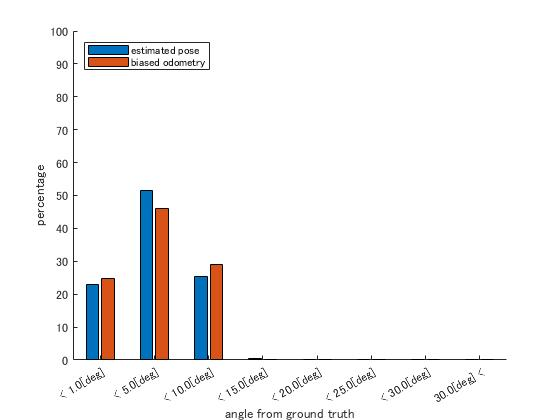
\includegraphics[width=110mm]{./picture/mesh_s8_rpy.jpg}
  \end{center}
  \caption{Sequence08における提案手法での角度推定精度}
  \label{fig:mesh_sequence08_RPY}
 \end{minipage}
\end{figure}

\begin{figure}[htbp]
 \begin{minipage}{1.0\hsize}
  \begin{center}
   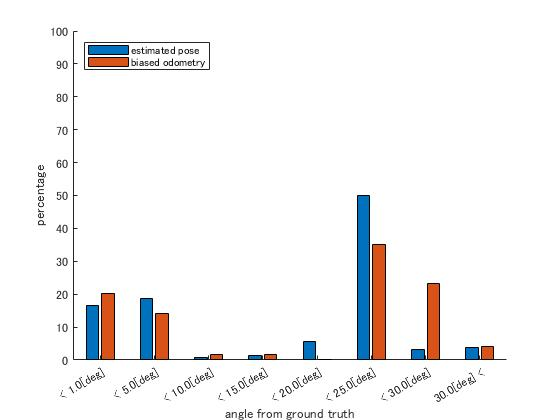
\includegraphics[width=110mm]{./picture/point_s8_rpy.jpg}
  \end{center}
  \caption{Sequence08における比較手法での角度推定精度}
  \label{fig:point_sequence08_RPY}
 \end{minipage}
\end{figure}


\subsection{尤度算出の評価}\label{sec:verify_likelihood}

%\subsubsection{水平変化に対する評価}

%\subsubsection{角度変化に対する評価}

\subsubsection{先行研究との評価}
提案手法における尤度算出の有効性を示すために, 時刻$t$における真の位置$x_{t}^{*}$からみたメッシュ地図と点群地図の風景をそれぞれ画像化してセグメンテーションされたカメラ画像$z_{t}$と比較, セマンティックなクラスが一致したピクセルの数を計測した. Sequence00の中から異なる13の位置を記録して先程述べた手法により比較を行った. この時の13の位置は図\ref{fig:sequence00_place}のとおりである. 全ピクセルの内何\%が一致していると判断されたかの結果を表\ref{tab:cmp_calc_likelihood}に示す. なお, 実験にあたり表\ref{tab:MCL_parameter}のimagedownwidthとimagedownheightを1.0に調整した. また, 各位置におけるカメラ画像, セグメンテーションされた画像, メッシュ地図, 点群地図, メッシュ地図と点群地図においてクラスが一致していると判断されたピクセルのみを抽出した画像を図\ref{fig:place1}から図\ref{fig:place13}にかけて示す. 

\begin{table}[htbp]
\begin{center}
\caption{メッシュ地図と点群地図での尤度算出の比較}
  \begin{tabular}{|c|r|r|} \hline
    地点 & メッシュ地図(\%) & 点群地図(\%)\\ \hline
    1 & 22.3 & 4.0 \\ \hline
    2 & 11.1 & 2.4 \\ \hline
    3 & 25.1 & 8.1 \\ \hline
    4 & 41.2 & 5.8 \\ \hline
    5 & 27.4 & 3.9 \\ \hline
    6 & 26.6 & 2.8 \\ \hline
    7 & 25.8 & 5.0 \\ \hline
    8 & 36.5 & 5.1 \\ \hline
    9 & 30.8 & 5.8 \\ \hline
    10 & 13.2 & 1.5 \\ \hline
    11 & 14.0 & 1.8 \\ \hline
    12 & 17.3 & 2.3 \\ \hline
    13 & 30.3 & 4.5 \\ \hline

  \end{tabular}
  \label{tab:cmp_calc_likelihood}
\end{center}
\end{table}

\begin{figure}[htpb]
\begin{minipage}[b]{1.0\hsize}
\begin{center}
    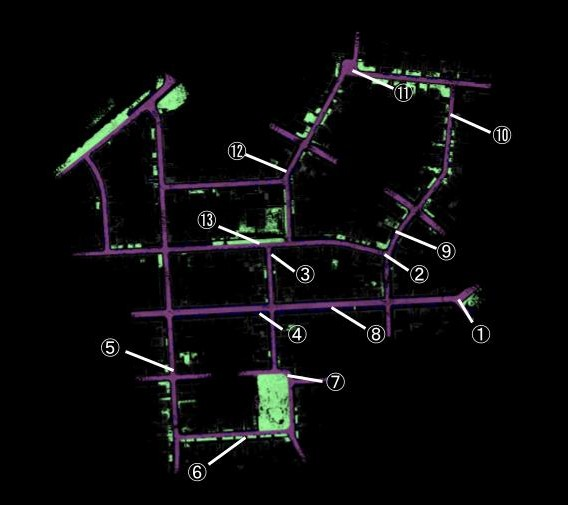
\includegraphics[width=120mm]{./picture/sequence00_pointmap.jpg}
\end{center}
\caption{尤度算出の検証において選定された地点}
\label{fig:sequence00_place}
\end{minipage}
\end{figure}

\begin{figure}[htbp]
 \begin{minipage}[b]{0.50\hsize}
 \begin{center}
  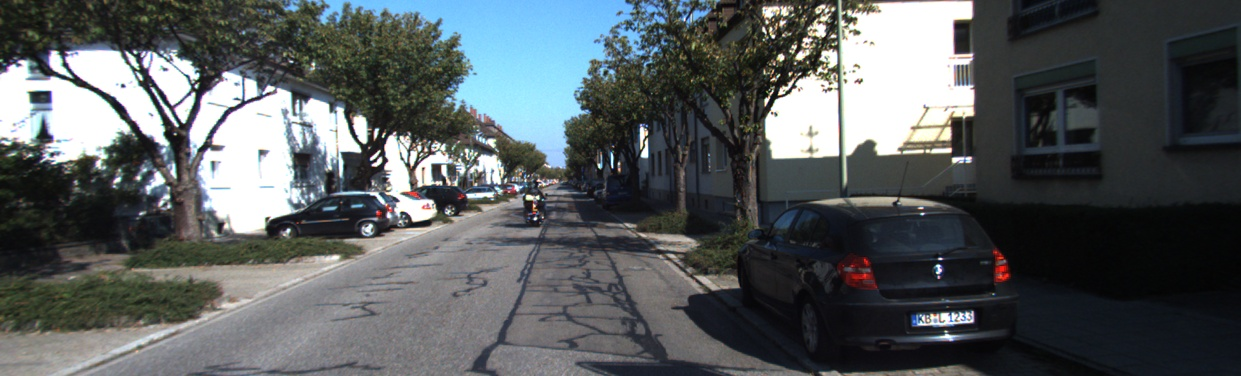
\includegraphics[keepaspectratio, scale=0.18]{./picture/bgrimage/bgrimage0.jpg}
  \subcaption{カメラ画像}
  \end{center}
 \end{minipage}
 \begin{minipage}[b]{0.5\hsize}
 \begin{center}
  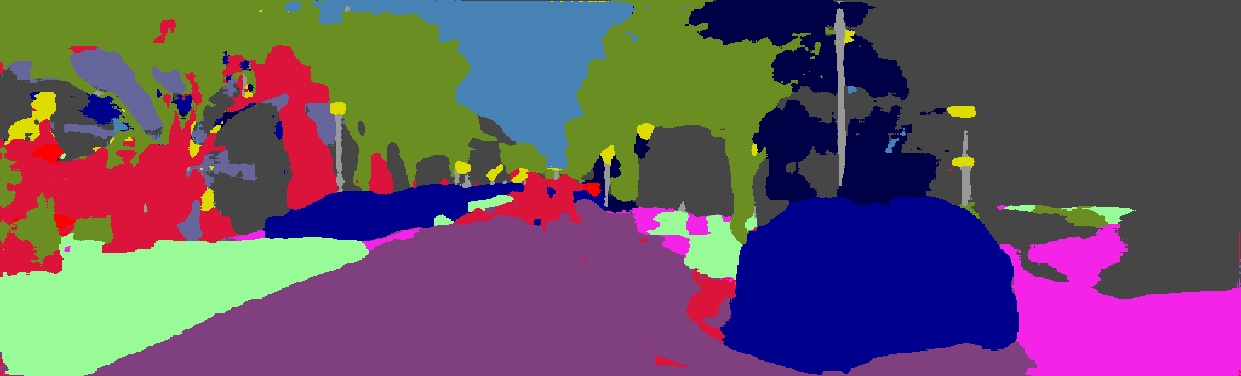
\includegraphics[keepaspectratio, scale=0.18]{./picture/segimage/image0.jpg}
  \subcaption{セグメンテーションされた画像}
  \end{center}
 \end{minipage} \\
 \begin{minipage}[b]{0.50\hsize}
 \begin{center}
  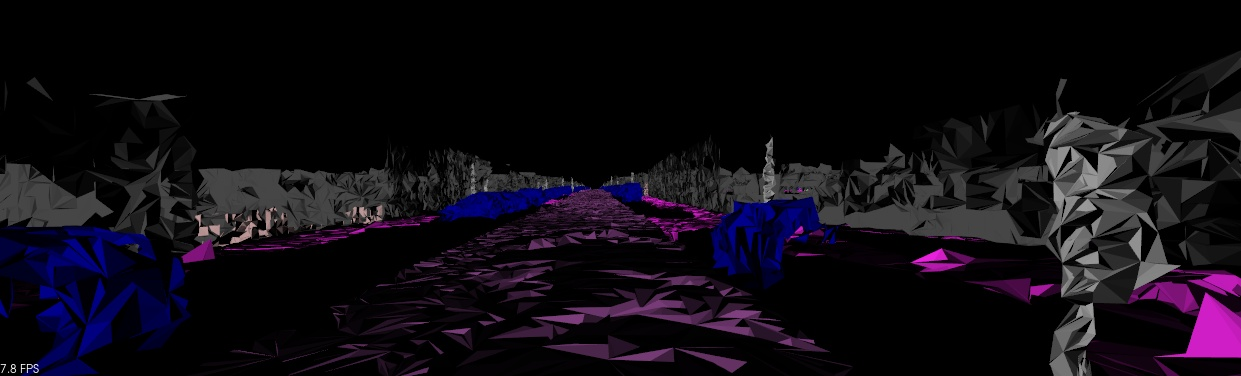
\includegraphics[keepaspectratio, scale=0.18]{./picture/mesh_map_image/image0.jpg}
  \subcaption{メッシュ地図}
  \end{center}
 \end{minipage}
 \begin{minipage}[b]{0.50\hsize}
 \begin{center}
  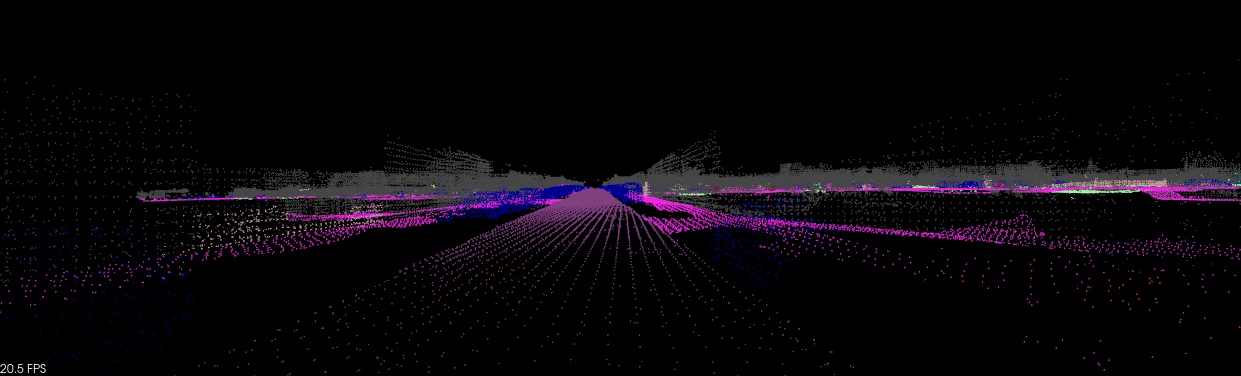
\includegraphics[keepaspectratio, scale=0.18]{./picture/point_map_image/image0.jpg}
  \subcaption{点群地図}
  \end{center}
 \end{minipage} \\
  \begin{minipage}[b]{0.50\hsize}
 \begin{center}
  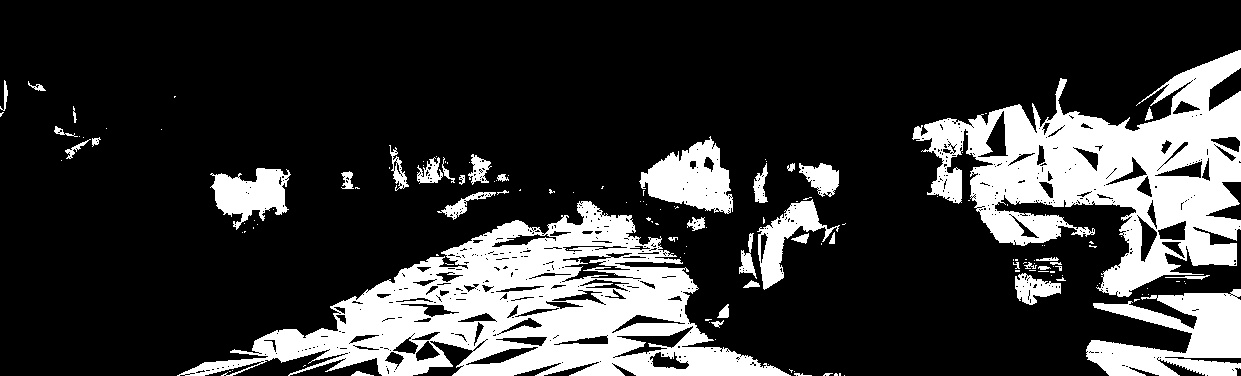
\includegraphics[keepaspectratio, scale=0.18]{./picture/valued_mesh_map_image/image0.jpg}
  \subcaption{メッシュ地図にてクラスが一致したピクセル}
  \end{center}
 \end{minipage}
 \begin{minipage}[b]{0.50\hsize}
 \begin{center}
  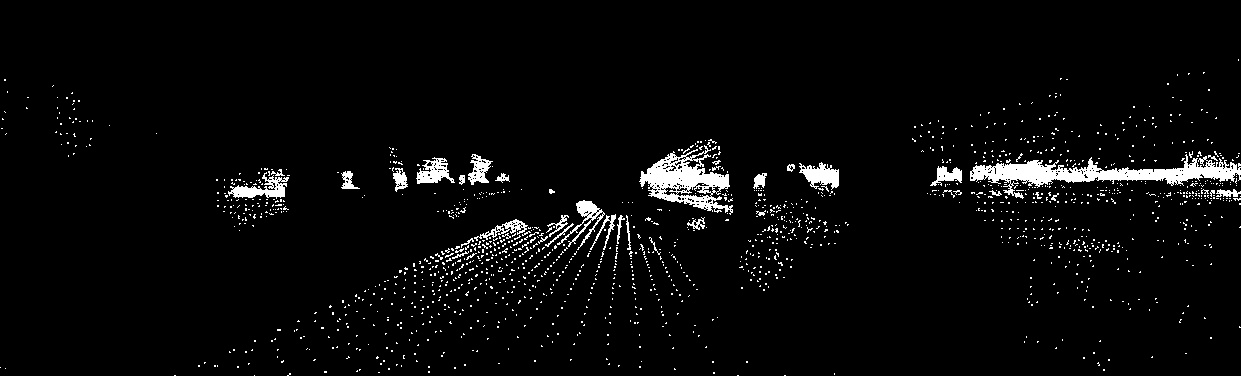
\includegraphics[keepaspectratio, scale=0.18]{./picture/valued_point_map_image/image0.jpg}
  \subcaption{点群地図にてクラスが一致したピクセル}
  \end{center}
 \end{minipage}
 \caption{位置1でのカメラ画像, セグメンテーションされた画像, メッシュ地図, 点群地図}\label{fig:place1}
\end{figure}

\par

\begin{figure}[htbp]
 \begin{minipage}[b]{0.50\hsize}
 \begin{center}
  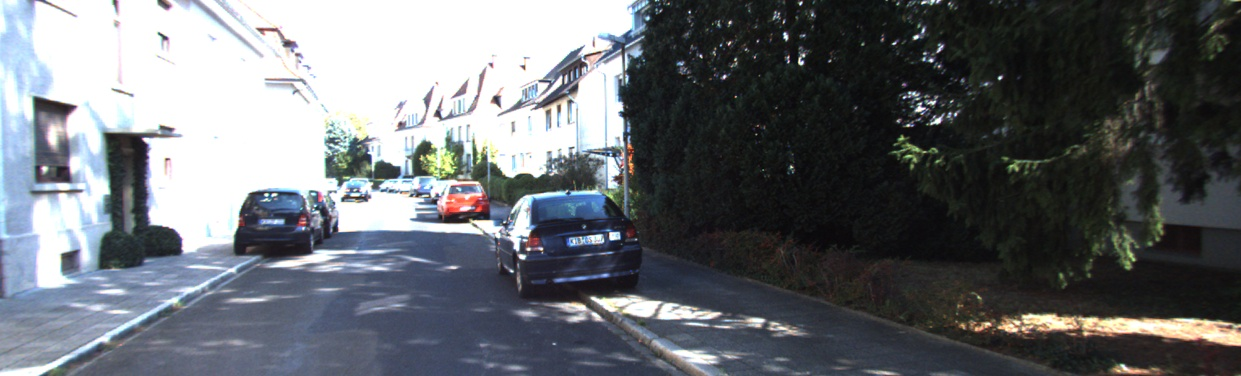
\includegraphics[keepaspectratio, scale=0.18]{./picture/bgrimage/bgrimage1.jpg}
  \subcaption{カメラ画像}
  \end{center}
 \end{minipage}
 \begin{minipage}[b]{0.5\hsize}
 \begin{center}
  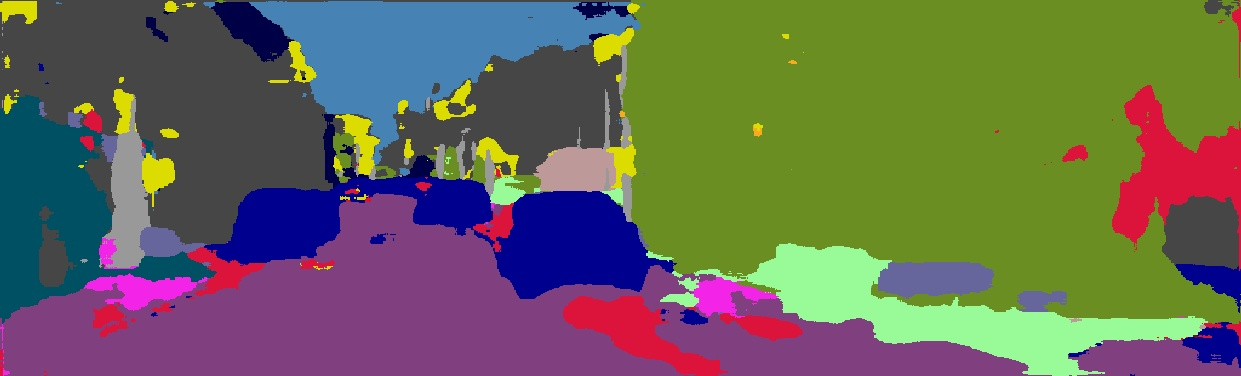
\includegraphics[keepaspectratio, scale=0.18]{./picture/segimage/image1.jpg}
  \subcaption{セグメンテーションされた画像}
  \end{center}
 \end{minipage} \\
 \begin{minipage}[b]{0.50\hsize}
 \begin{center}
  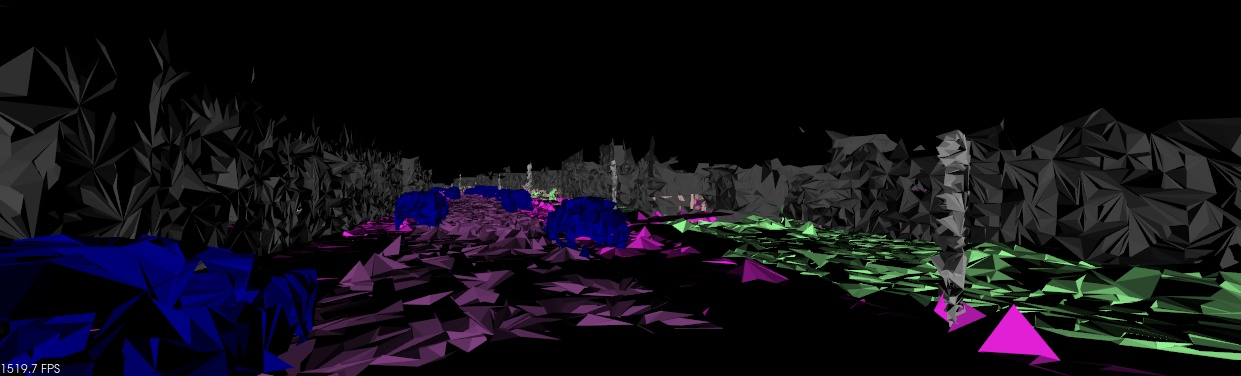
\includegraphics[keepaspectratio, scale=0.18]{./picture/mesh_map_image/image1.jpg}
  \subcaption{メッシュ地図}
  \end{center}
 \end{minipage}
 \begin{minipage}[b]{0.50\hsize}
 \begin{center}
  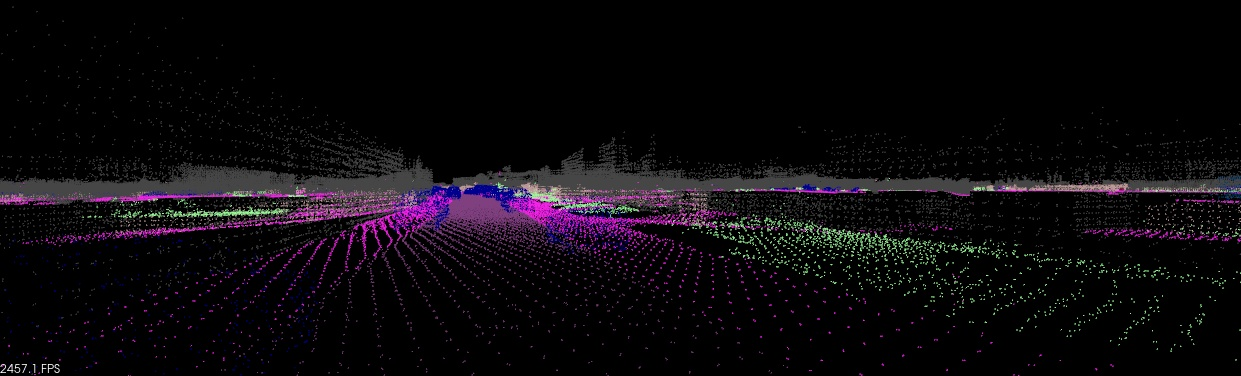
\includegraphics[keepaspectratio, scale=0.18]{./picture/point_map_image/image1.jpg}
  \subcaption{点群地図}
  \end{center}
 \end{minipage} \\
   \begin{minipage}[b]{0.50\hsize}
 \begin{center}
  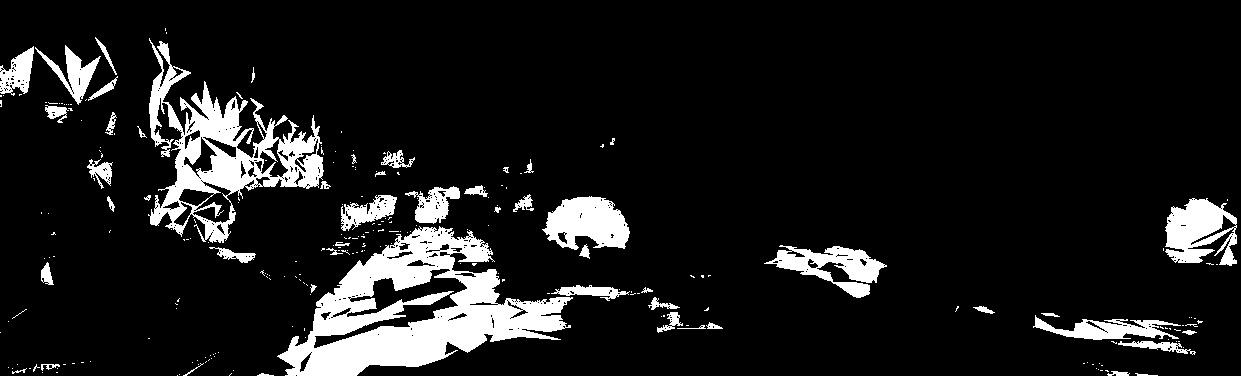
\includegraphics[keepaspectratio, scale=0.18]{./picture/valued_mesh_map_image/image1.jpg}
  \subcaption{メッシュ地図にてクラスが一致したピクセル}
  \end{center}
 \end{minipage}
 \begin{minipage}[b]{0.50\hsize}
 \begin{center}
  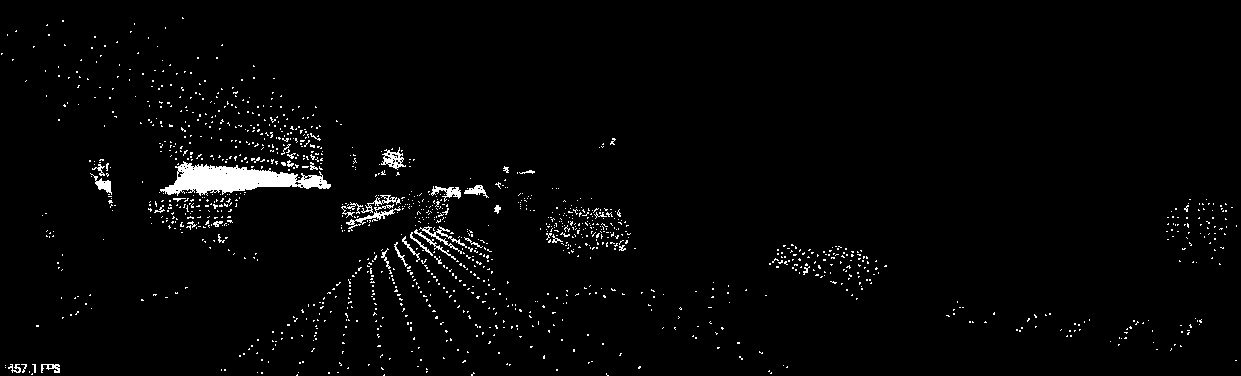
\includegraphics[keepaspectratio, scale=0.18]{./picture/valued_point_map_image/image1.jpg}
  \subcaption{点群地図にてクラスが一致したピクセル}
  \end{center}
 \end{minipage}
 \caption{位置2でのカメラ画像, セグメンテーションされた画像, メッシュ地図, 点群地図}\label{fig:place2}
\end{figure}

\begin{figure}[htbp]
 \begin{minipage}[b]{0.50\hsize}
 \begin{center}
  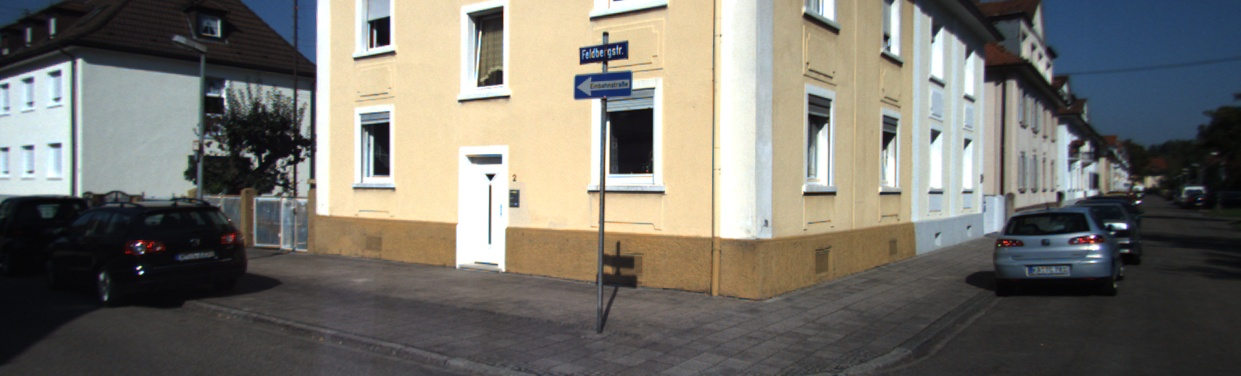
\includegraphics[keepaspectratio, scale=0.18]{./picture/bgrimage/bgrimage2.jpg}
  \subcaption{カメラ画像}
  \end{center}
 \end{minipage}
 \begin{minipage}[b]{0.5\hsize}
 \begin{center}
  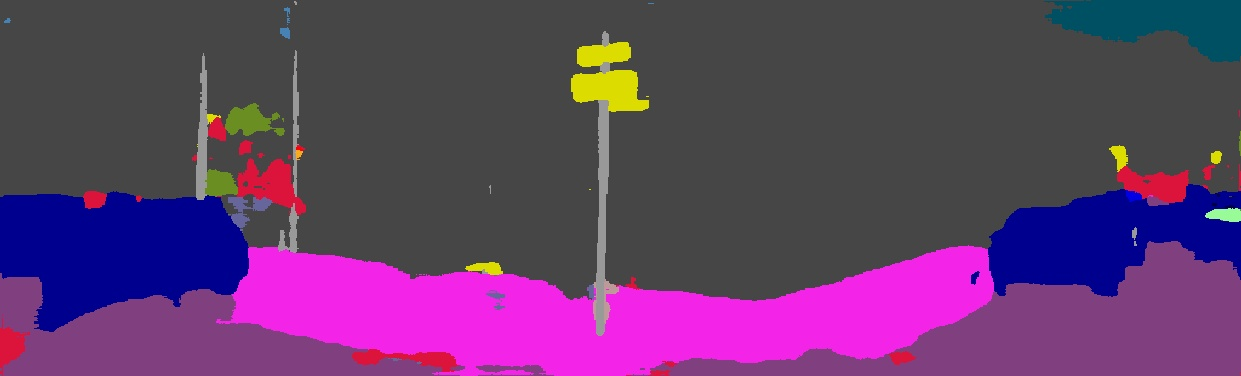
\includegraphics[keepaspectratio, scale=0.18]{./picture/segimage/image2.jpg}
  \subcaption{セグメンテーションされた画像}
  \end{center}
 \end{minipage} \\
 \begin{minipage}[b]{0.50\hsize}
 \begin{center}
  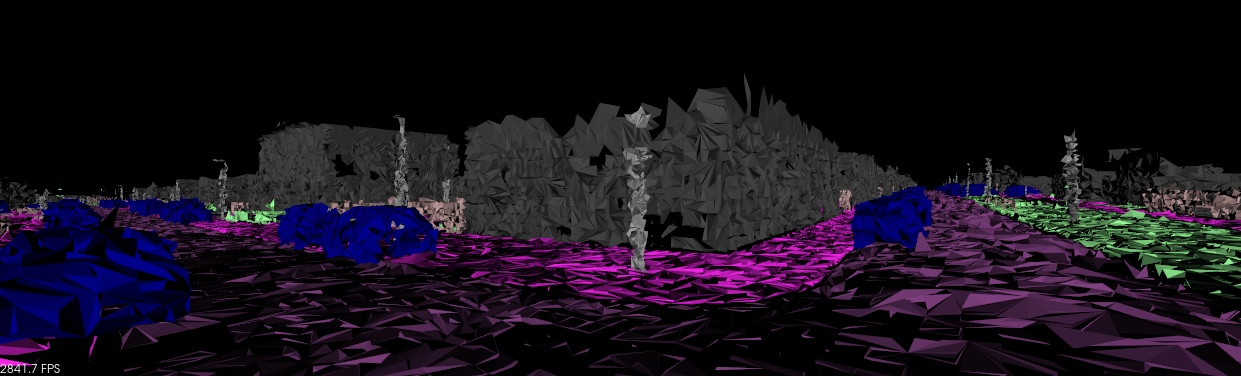
\includegraphics[keepaspectratio, scale=0.18]{./picture/mesh_map_image/image2.jpg}
  \subcaption{メッシュ地図}
  \end{center}
 \end{minipage}
 \begin{minipage}[b]{0.50\hsize}
 \begin{center}
  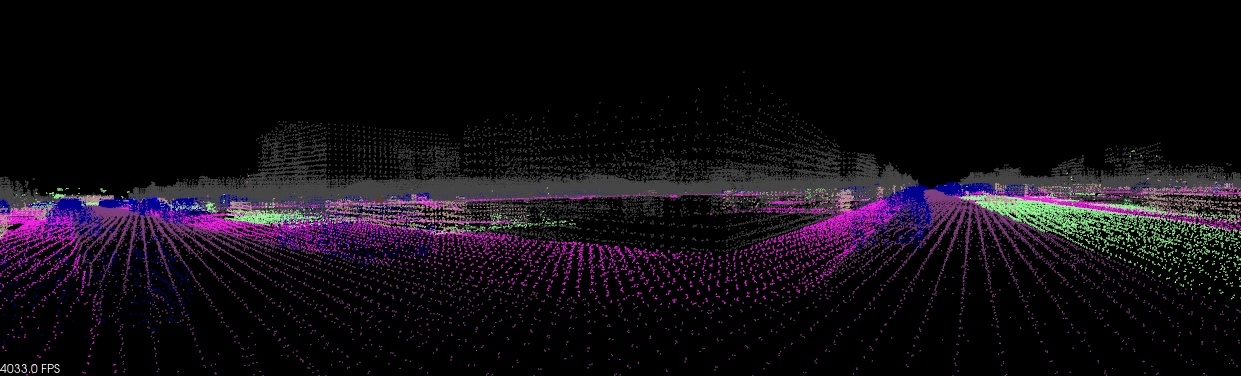
\includegraphics[keepaspectratio, scale=0.18]{./picture/point_map_image/image2.jpg}
  \subcaption{点群地図}
  \end{center}
 \end{minipage} \\
   \begin{minipage}[b]{0.50\hsize}
 \begin{center}
  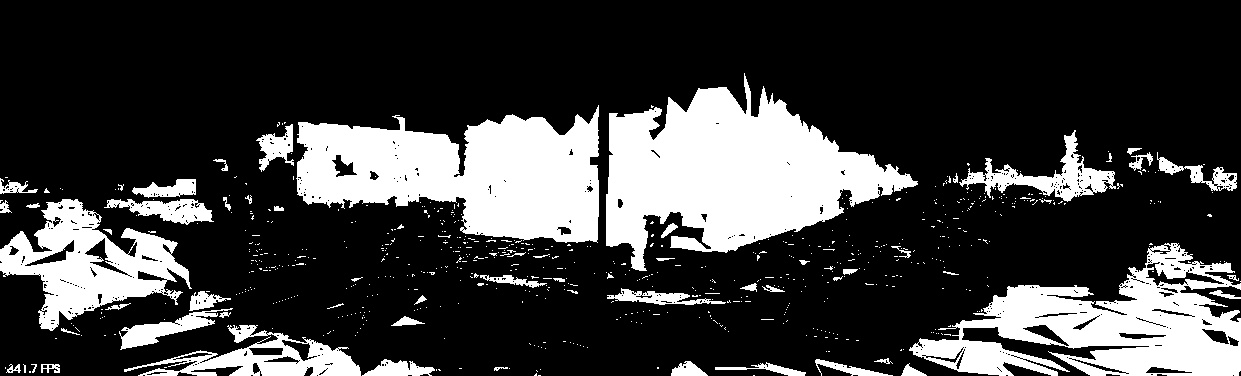
\includegraphics[keepaspectratio, scale=0.18]{./picture/valued_mesh_map_image/image2.jpg}
  \subcaption{メッシュ地図にてクラスが一致したピクセル}
  \end{center}
 \end{minipage}
 \begin{minipage}[b]{0.50\hsize}
 \begin{center}
  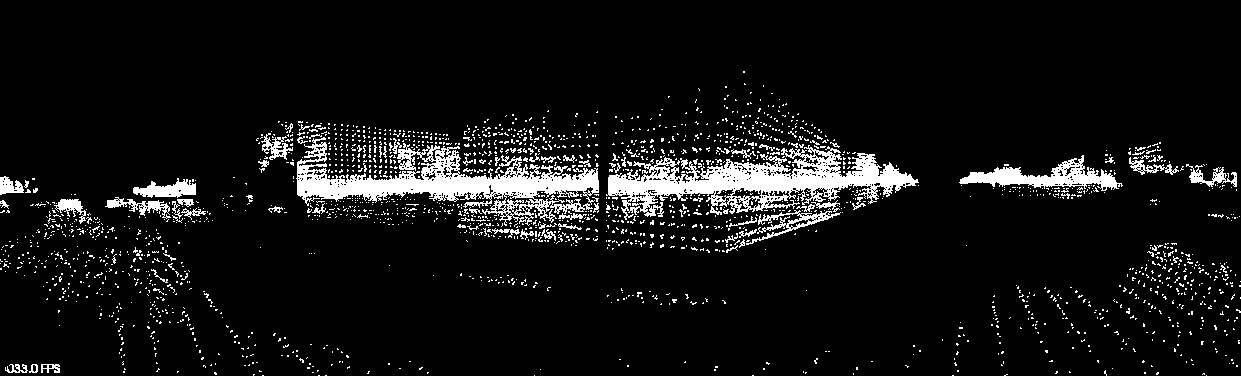
\includegraphics[keepaspectratio, scale=0.18]{./picture/valued_point_map_image/image2.jpg}
  \subcaption{点群地図にてクラスが一致したピクセル}
  \end{center}
 \end{minipage}
 \caption{位置3でのカメラ画像, セグメンテーションされた画像, メッシュ地図, 点群地図}\label{fig:place3}
\end{figure}


\begin{figure}[htbp]
 \begin{minipage}[b]{0.50\hsize}
 \begin{center}
  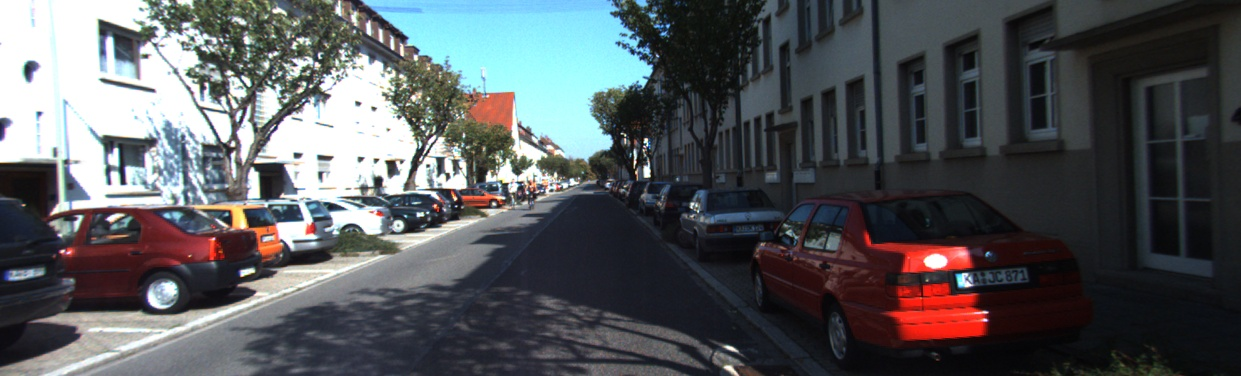
\includegraphics[keepaspectratio, scale=0.18]{./picture/bgrimage/bgrimage3.jpg}
  \subcaption{カメラ画像}
  \end{center}
 \end{minipage}
 \begin{minipage}[b]{0.5\hsize}
 \begin{center}
  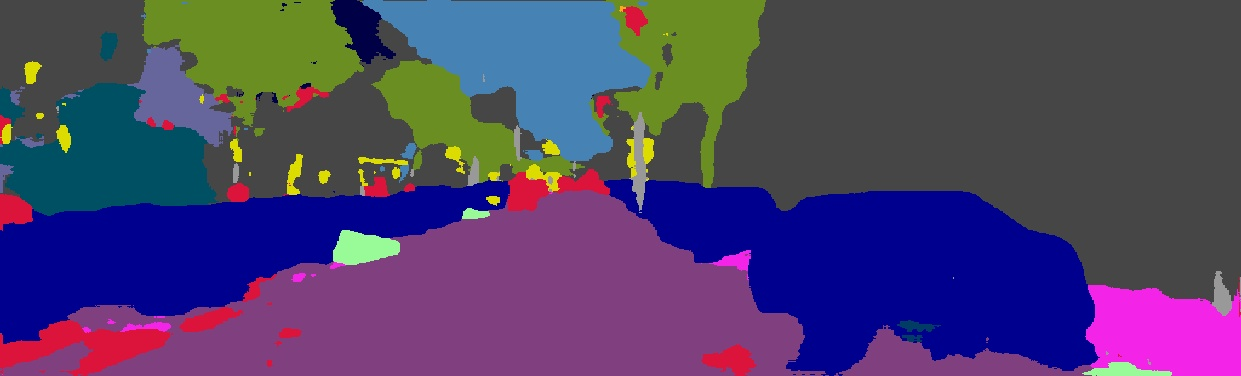
\includegraphics[keepaspectratio, scale=0.18]{./picture/segimage/image3.jpg}
  \subcaption{セグメンテーションされた画像}
  \end{center}
 \end{minipage} \\
 \begin{minipage}[b]{0.50\hsize}
 \begin{center}
  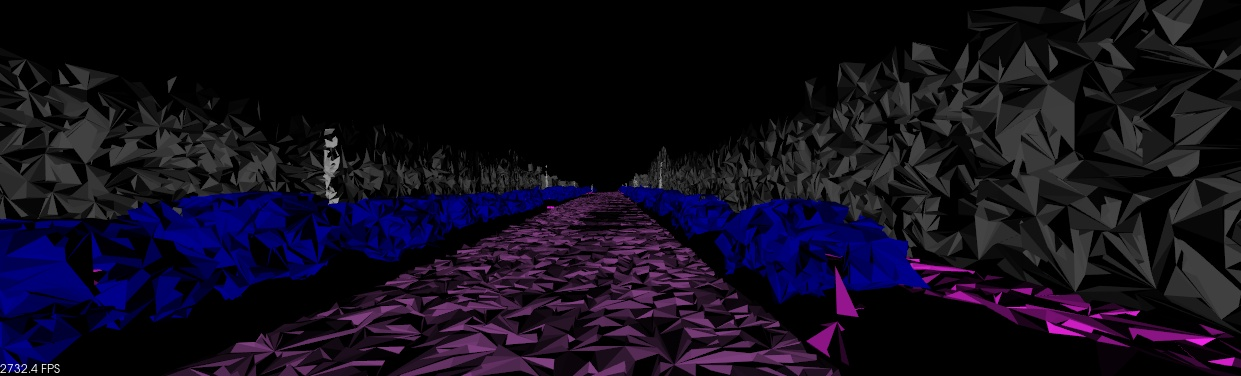
\includegraphics[keepaspectratio, scale=0.18]{./picture/mesh_map_image/image3.jpg}
  \subcaption{メッシュ地図}
  \end{center}
 \end{minipage}
 \begin{minipage}[b]{0.50\hsize}
 \begin{center}
  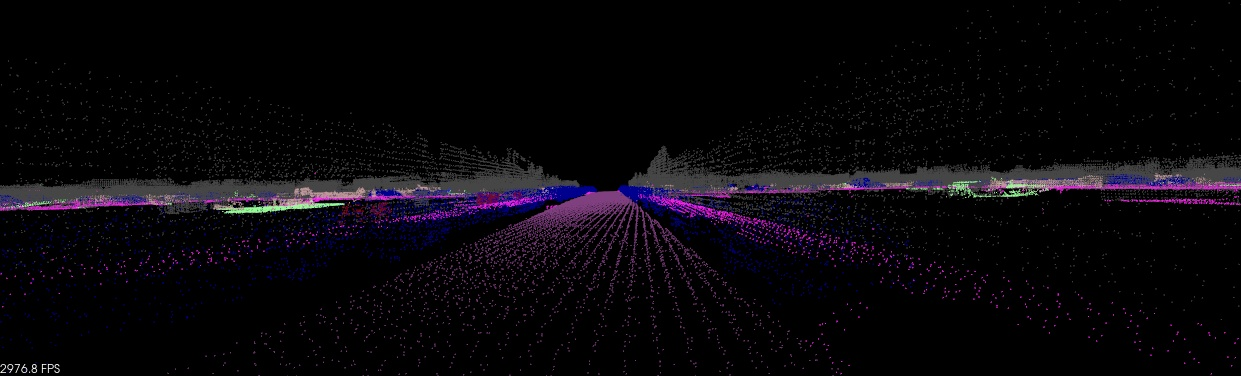
\includegraphics[keepaspectratio, scale=0.18]{./picture/point_map_image/image3.jpg}
  \subcaption{点群地図}
  \end{center}
 \end{minipage}\\
  \begin{minipage}[b]{0.50\hsize}
 \begin{center}
  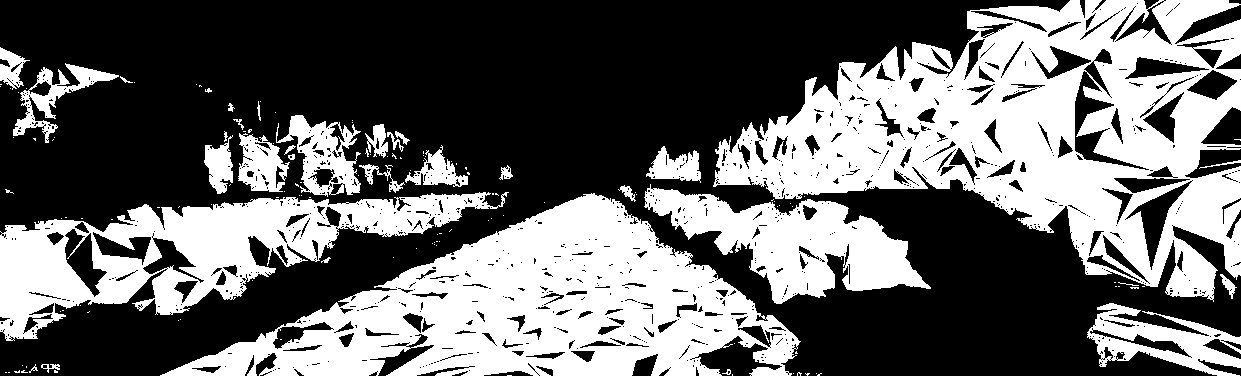
\includegraphics[keepaspectratio, scale=0.18]{./picture/valued_mesh_map_image/image3.jpg}
  \subcaption{メッシュ地図にてクラスが一致したピクセル}
  \end{center}
 \end{minipage}
 \begin{minipage}[b]{0.50\hsize}
 \begin{center}
  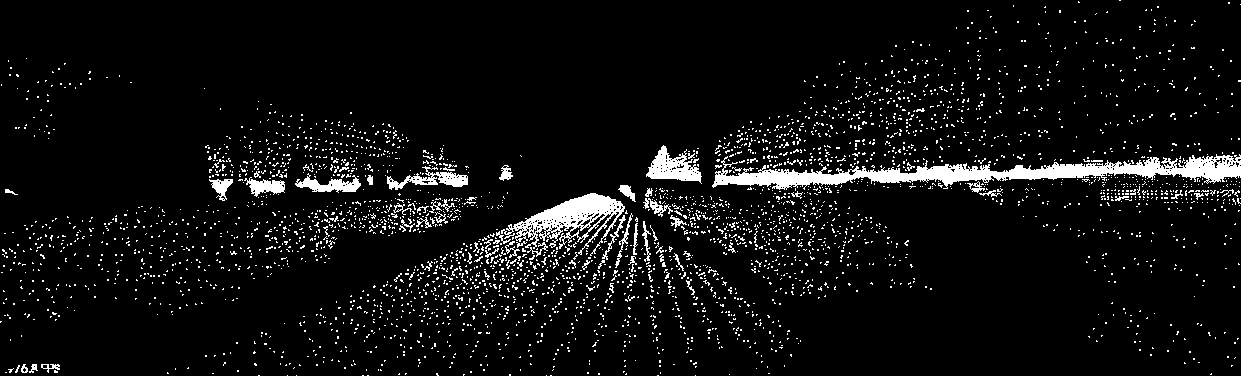
\includegraphics[keepaspectratio, scale=0.18]{./picture/valued_point_map_image/image3.jpg}
  \subcaption{点群地図にてクラスが一致したピクセル}
  \end{center}
 \end{minipage}
 \caption{位置4でのカメラ画像, セグメンテーションされた画像, メッシュ地図, 点群地図}\label{fig:place4}
\end{figure}

\begin{figure}[htbp]
 \begin{minipage}[b]{0.50\hsize}
 \begin{center}
  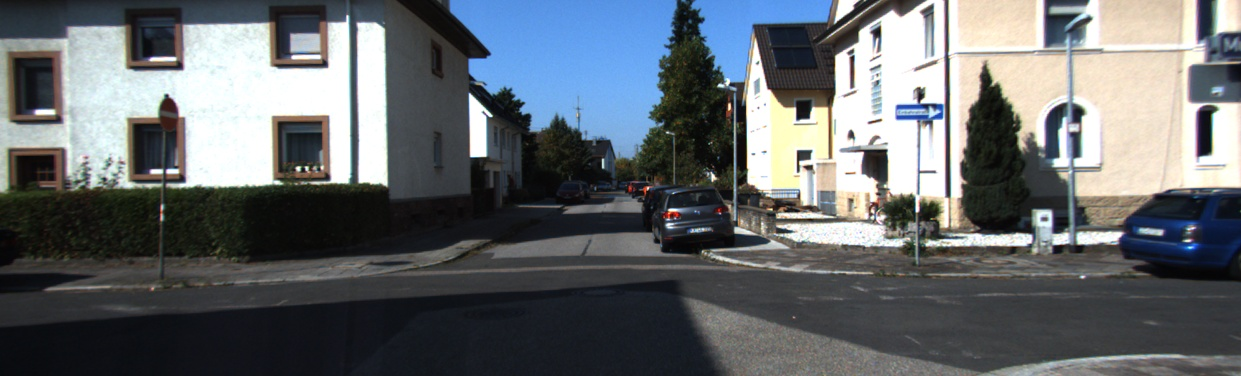
\includegraphics[keepaspectratio, scale=0.18]{./picture/bgrimage/bgrimage4.jpg}
  \subcaption{カメラ画像}
  \end{center}
 \end{minipage}
 \begin{minipage}[b]{0.5\hsize}
 \begin{center}
  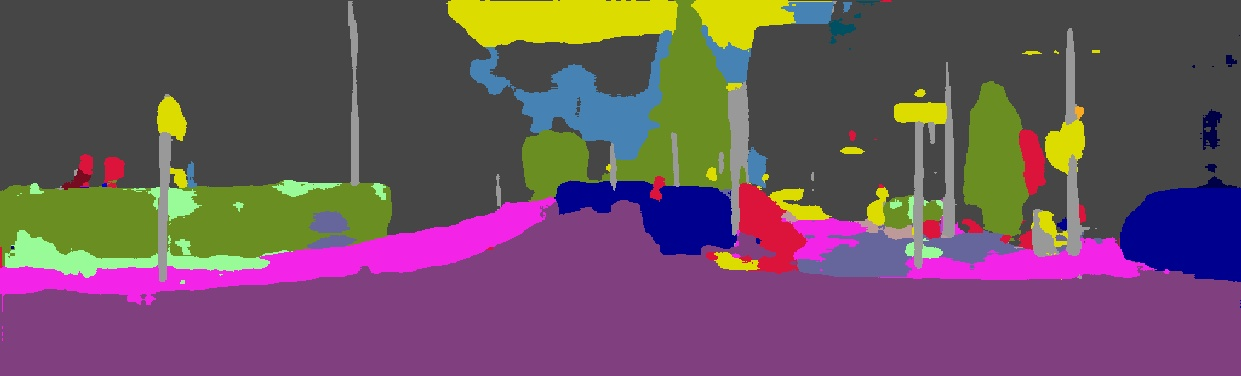
\includegraphics[keepaspectratio, scale=0.18]{./picture/segimage/image4.jpg}
  \subcaption{セグメンテーションされた画像}
  \end{center}
 \end{minipage} \\
 \begin{minipage}[b]{0.50\hsize}
 \begin{center}
  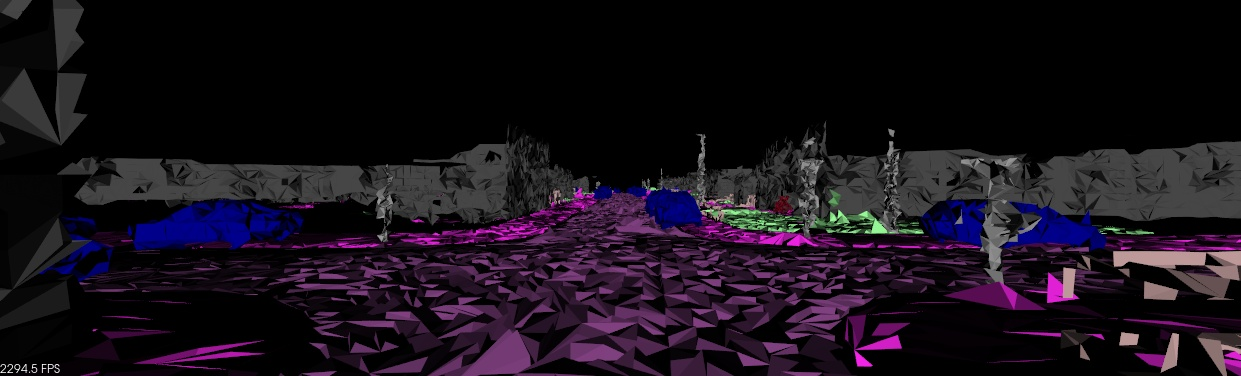
\includegraphics[keepaspectratio, scale=0.18]{./picture/mesh_map_image/image4.jpg}
  \subcaption{メッシュ地図}
  \end{center}
 \end{minipage}
 \begin{minipage}[b]{0.50\hsize}
 \begin{center}
  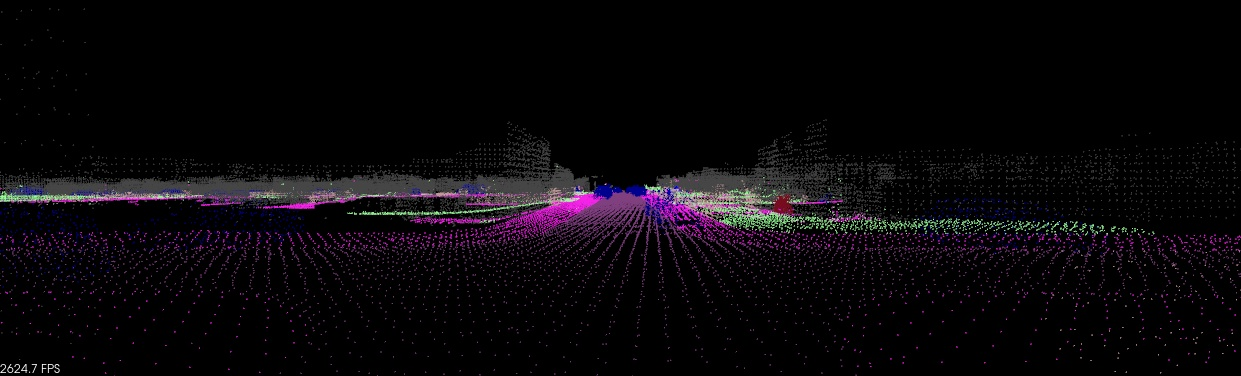
\includegraphics[keepaspectratio, scale=0.18]{./picture/point_map_image/image4.jpg}
  \subcaption{点群地図}
  \end{center}
 \end{minipage}\\
  \begin{minipage}[b]{0.50\hsize}
 \begin{center}
  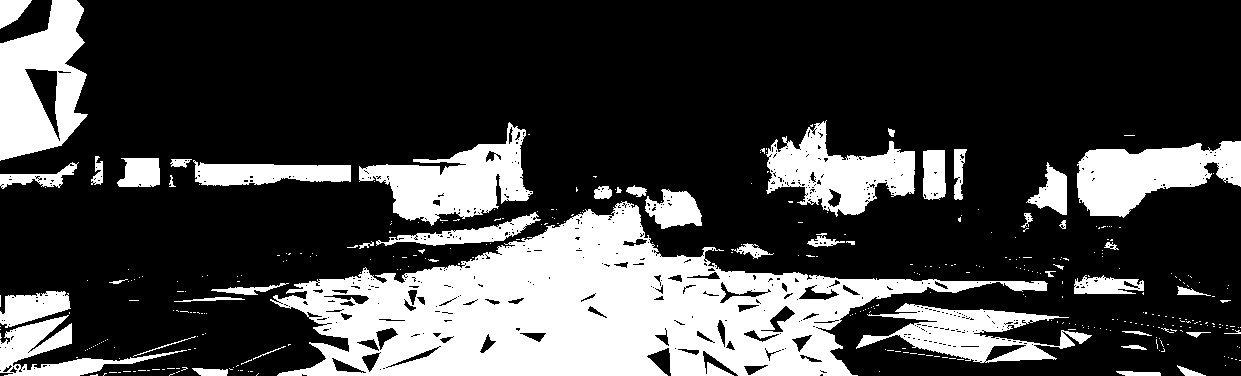
\includegraphics[keepaspectratio, scale=0.18]{./picture/valued_mesh_map_image/image4.jpg}
  \subcaption{メッシュ地図にてクラスが一致したピクセル}
  \end{center}
 \end{minipage}
 \begin{minipage}[b]{0.50\hsize}
 \begin{center}
  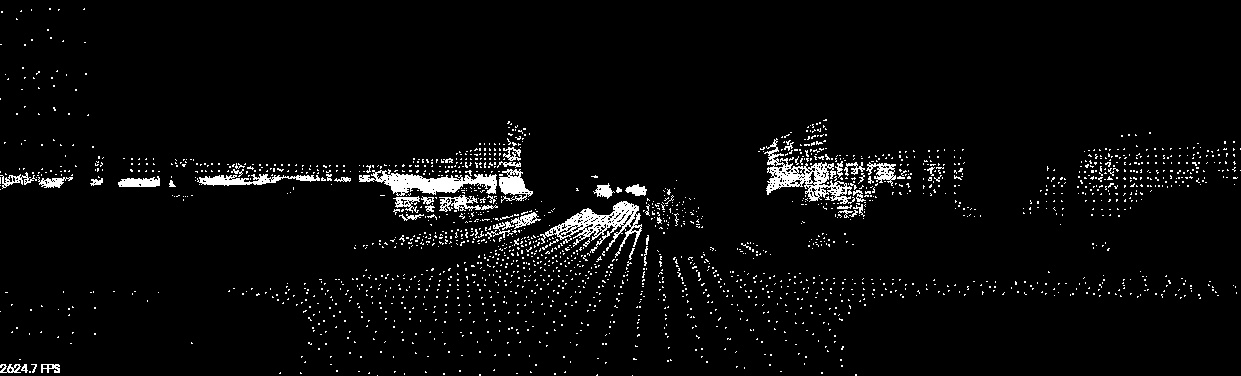
\includegraphics[keepaspectratio, scale=0.18]{./picture/valued_point_map_image/image4.jpg}
  \subcaption{点群地図にてクラスが一致したピクセル}
  \end{center}
 \end{minipage}
 \caption{位置5でのカメラ画像, セグメンテーションされた画像, メッシュ地図, 点群地図}\label{fig:place5}
\end{figure}

\begin{figure}[htbp]
 \begin{minipage}[b]{0.50\hsize}
 \begin{center}
  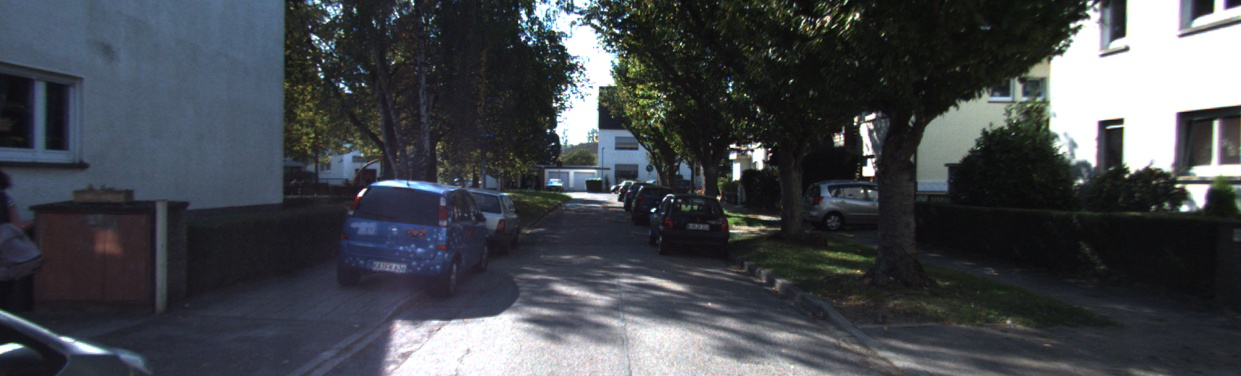
\includegraphics[keepaspectratio, scale=0.18]{./picture/bgrimage/bgrimage5.jpg}
  \subcaption{カメラ画像}
  \end{center}
 \end{minipage}
 \begin{minipage}[b]{0.5\hsize}
 \begin{center}
  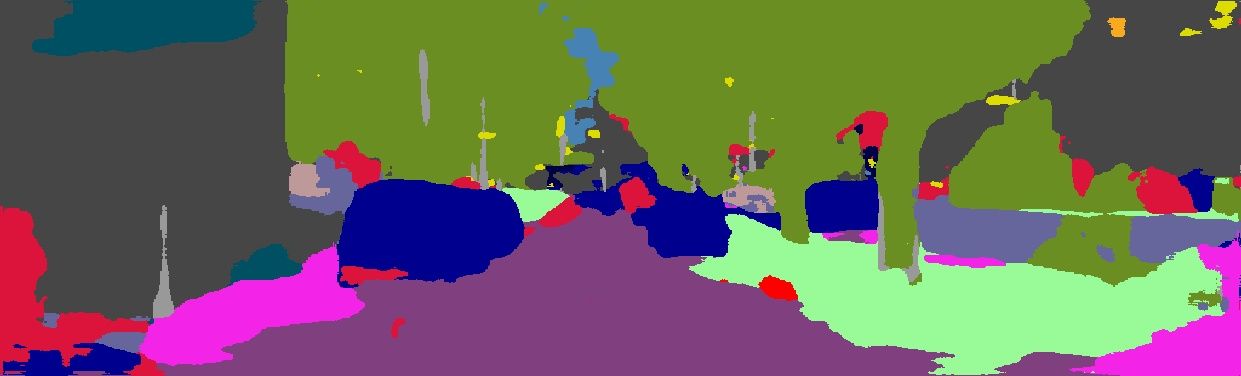
\includegraphics[keepaspectratio, scale=0.18]{./picture/segimage/image5.jpg}
  \subcaption{セグメンテーションされた画像}
  \end{center}
 \end{minipage} \\
 \begin{minipage}[b]{0.50\hsize}
 \begin{center}
  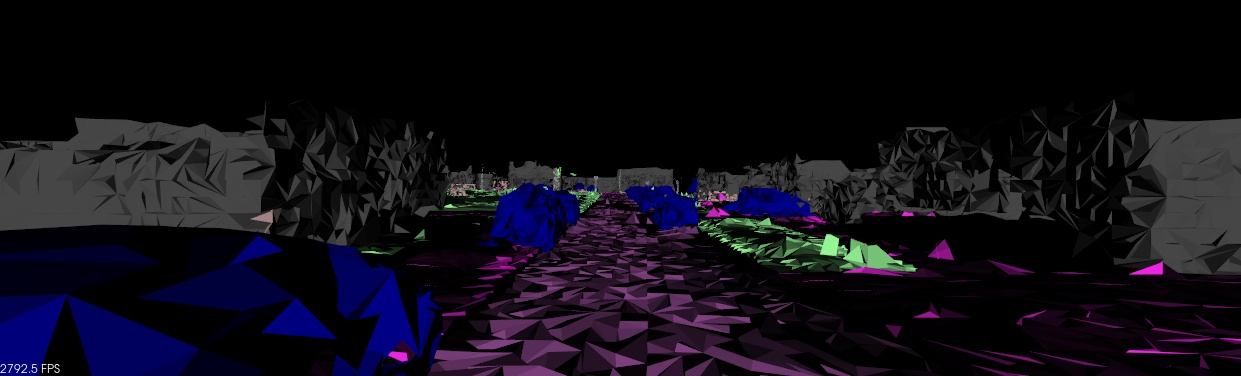
\includegraphics[keepaspectratio, scale=0.18]{./picture/mesh_map_image/image5.jpg}
  \subcaption{メッシュ地図}
  \end{center}
 \end{minipage}
 \begin{minipage}[b]{0.50\hsize}
 \begin{center}
  \includegraphics[keepaspectratio, scale=0.18]{./picture/point_map_image/image5.jpg}
  \subcaption{点群地図}
  \end{center}
 \end{minipage} \\
  \begin{minipage}[b]{0.50\hsize}
 \begin{center}
  \includegraphics[keepaspectratio, scale=0.18]{./picture/valued_mesh_map_image/image5.jpg}
  \subcaption{メッシュ地図にてクラスが一致したピクセル}
  \end{center}
 \end{minipage}
 \begin{minipage}[b]{0.50\hsize}
 \begin{center}
  \includegraphics[keepaspectratio, scale=0.18]{./picture/valued_point_map_image/image5.jpg}
  \subcaption{点群地図にてクラスが一致したピクセル}
  \end{center}
 \end{minipage}
 \caption{位置6でのカメラ画像, セグメンテーションされた画像, メッシュ地図, 点群地図}\label{fig:place6}
\end{figure}

\begin{figure}[htbp]
 \begin{minipage}[b]{0.50\hsize}
 \begin{center}
  \includegraphics[keepaspectratio, scale=0.18]{./picture/bgrimage/bgrimage6.jpg}
  \subcaption{カメラ画像}
  \end{center}
 \end{minipage}
 \begin{minipage}[b]{0.5\hsize}
 \begin{center}
  \includegraphics[keepaspectratio, scale=0.18]{./picture/segimage/image6.jpg}
  \subcaption{セグメンテーションされた画像}
  \end{center}
 \end{minipage} \\
 \begin{minipage}[b]{0.50\hsize}
 \begin{center}
  \includegraphics[keepaspectratio, scale=0.18]{./picture/mesh_map_image/image6.jpg}
  \subcaption{メッシュ地図}
  \end{center}
 \end{minipage}
 \begin{minipage}[b]{0.50\hsize}
 \begin{center}
  \includegraphics[keepaspectratio, scale=0.18]{./picture/point_map_image/image6.jpg}
  \subcaption{点群地図}
  \end{center}
 \end{minipage} \\
  \begin{minipage}[b]{0.50\hsize}
 \begin{center}
  \includegraphics[keepaspectratio, scale=0.18]{./picture/valued_mesh_map_image/image6.jpg}
  \subcaption{メッシュ地図にてクラスが一致したピクセル}
  \end{center}
 \end{minipage}
 \begin{minipage}[b]{0.50\hsize}
 \begin{center}
  \includegraphics[keepaspectratio, scale=0.18]{./picture/valued_point_map_image/image6.jpg}
  \subcaption{点群地図にてクラスが一致したピクセル}
  \end{center}
 \end{minipage}
 \caption{位置7でのカメラ画像, セグメンテーションされた画像, メッシュ地図, 点群地図}\label{fig:place7}
\end{figure}

\begin{figure}[htbp]
 \begin{minipage}[b]{0.50\hsize}
 \begin{center}
  \includegraphics[keepaspectratio, scale=0.18]{./picture/bgrimage/bgrimage7.jpg}
  \subcaption{カメラ画像}
  \end{center}
 \end{minipage}
 \begin{minipage}[b]{0.5\hsize}
 \begin{center}
  \includegraphics[keepaspectratio, scale=0.18]{./picture/segimage/image7.jpg}
  \subcaption{セグメンテーションされた画像}
  \end{center}
 \end{minipage} \\
 \begin{minipage}[b]{0.50\hsize}
 \begin{center}
  \includegraphics[keepaspectratio, scale=0.18]{./picture/mesh_map_image/image7.jpg}
  \subcaption{メッシュ地図}
  \end{center}
 \end{minipage}
 \begin{minipage}[b]{0.50\hsize}
 \begin{center}
  \includegraphics[keepaspectratio, scale=0.18]{./picture/point_map_image/image7.jpg}
  \subcaption{点群地図}
  \end{center}
 \end{minipage} \\
  \begin{minipage}[b]{0.50\hsize}
 \begin{center}
  \includegraphics[keepaspectratio, scale=0.18]{./picture/valued_mesh_map_image/image7.jpg}
  \subcaption{メッシュ地図にてクラスが一致したピクセル}
  \end{center}
 \end{minipage}
 \begin{minipage}[b]{0.50\hsize}
 \begin{center}
  \includegraphics[keepaspectratio, scale=0.18]{./picture/valued_point_map_image/image7.jpg}
  \subcaption{点群地図にてクラスが一致したピクセル}
  \end{center}
 \end{minipage}
 \caption{位置8でのカメラ画像, セグメンテーションされた画像, メッシュ地図, 点群地図}\label{fig:place8}
\end{figure}

\begin{figure}[htbp]
 \begin{minipage}[b]{0.50\hsize}
 \begin{center}
  \includegraphics[keepaspectratio, scale=0.18]{./picture/bgrimage/bgrimage8.jpg}
  \subcaption{カメラ画像}
  \end{center}
 \end{minipage}
 \begin{minipage}[b]{0.5\hsize}
 \begin{center}
  \includegraphics[keepaspectratio, scale=0.18]{./picture/segimage/image8.jpg}
  \subcaption{セグメンテーションされた画像}
  \end{center}
 \end{minipage} \\
 \begin{minipage}[b]{0.50\hsize}
 \begin{center}
  \includegraphics[keepaspectratio, scale=0.18]{./picture/mesh_map_image/image8.jpg}
  \subcaption{メッシュ地図}
  \end{center}
 \end{minipage}
 \begin{minipage}[b]{0.50\hsize}
 \begin{center}
  \includegraphics[keepaspectratio, scale=0.18]{./picture/point_map_image/image8.jpg}
  \subcaption{点群地図}
  \end{center}
 \end{minipage} \\
  \begin{minipage}[b]{0.50\hsize}
 \begin{center}
  \includegraphics[keepaspectratio, scale=0.18]{./picture/valued_mesh_map_image/image8.jpg}
  \subcaption{メッシュ地図にてクラスが一致したピクセル}
  \end{center}
 \end{minipage}
 \begin{minipage}[b]{0.50\hsize}
 \begin{center}
  \includegraphics[keepaspectratio, scale=0.18]{./picture/valued_point_map_image/image8.jpg}
  \subcaption{点群地図にてクラスが一致したピクセル}
  \end{center}
 \end{minipage}
 \caption{位置9でのカメラ画像, セグメンテーションされた画像, メッシュ地図, 点群地図}\label{fig:place9}
\end{figure}

\begin{figure}[htbp]
 \begin{minipage}[b]{0.50\hsize}
 \begin{center}
  \includegraphics[keepaspectratio, scale=0.18]{./picture/bgrimage/bgrimage9.jpg}
  \subcaption{カメラ画像}
  \end{center}
 \end{minipage}
 \begin{minipage}[b]{0.5\hsize}
 \begin{center}
  \includegraphics[keepaspectratio, scale=0.18]{./picture/segimage/image9.jpg}
  \subcaption{セグメンテーションされた画像}
  \end{center}
 \end{minipage} \\
 \begin{minipage}[b]{0.50\hsize}
 \begin{center}
  \includegraphics[keepaspectratio, scale=0.18]{./picture/mesh_map_image/image9.jpg}
  \subcaption{メッシュ地図}
  \end{center}
 \end{minipage}
 \begin{minipage}[b]{0.50\hsize}
 \begin{center}
  \includegraphics[keepaspectratio, scale=0.18]{./picture/point_map_image/image9.jpg}
  \subcaption{点群地図}
  \end{center}
 \end{minipage} \\
  \begin{minipage}[b]{0.50\hsize}
 \begin{center}
  \includegraphics[keepaspectratio, scale=0.18]{./picture/valued_mesh_map_image/image9.jpg}
  \subcaption{メッシュ地図にてクラスが一致したピクセル}
  \end{center}
 \end{minipage}
 \begin{minipage}[b]{0.50\hsize}
 \begin{center}
  \includegraphics[keepaspectratio, scale=0.18]{./picture/valued_point_map_image/image9.jpg}
  \subcaption{点群地図にてクラスが一致したピクセル}
  \end{center}
 \end{minipage}
 \caption{位置10でのカメラ画像, セグメンテーションされた画像, メッシュ地図, 点群地図}\label{fig:place10}
\end{figure}

\begin{figure}[htbp]
 \begin{minipage}[b]{0.50\hsize}
 \begin{center}
  \includegraphics[keepaspectratio, scale=0.18]{./picture/bgrimage/bgrimage10.jpg}
  \subcaption{カメラ画像}
  \end{center}
 \end{minipage}
 \begin{minipage}[b]{0.5\hsize}
 \begin{center}
  \includegraphics[keepaspectratio, scale=0.18]{./picture/segimage/image10.jpg}
  \subcaption{セグメンテーションされた画像}
  \end{center}
 \end{minipage} \\
 \begin{minipage}[b]{0.50\hsize}
 \begin{center}
  \includegraphics[keepaspectratio, scale=0.18]{./picture/mesh_map_image/image10.jpg}
  \subcaption{メッシュ地図}
  \end{center}
 \end{minipage}
 \begin{minipage}[b]{0.50\hsize}
 \begin{center}
  \includegraphics[keepaspectratio, scale=0.18]{./picture/point_map_image/image10.jpg}
  \subcaption{点群地図}
  \end{center}
 \end{minipage} \\
  \begin{minipage}[b]{0.50\hsize}
 \begin{center}
  \includegraphics[keepaspectratio, scale=0.18]{./picture/valued_mesh_map_image/image10.jpg}
  \subcaption{メッシュ地図にてクラスが一致したピクセル}
  \end{center}
 \end{minipage}
 \begin{minipage}[b]{0.50\hsize}
 \begin{center}
  \includegraphics[keepaspectratio, scale=0.18]{./picture/valued_point_map_image/image10.jpg}
  \subcaption{点群地図にてクラスが一致したピクセル}
  \end{center}
 \end{minipage}
 \caption{位置11でのカメラ画像, セグメンテーションされた画像, メッシュ地図, 点群地図}\label{fig:place11}
\end{figure}

\begin{figure}[htbp]
 \begin{minipage}[b]{0.50\hsize}
 \begin{center}
  \includegraphics[keepaspectratio, scale=0.18]{./picture/bgrimage/bgrimage11.jpg}
  \subcaption{カメラ画像}
  \end{center}
 \end{minipage}
 \begin{minipage}[b]{0.5\hsize}
 \begin{center}
  \includegraphics[keepaspectratio, scale=0.18]{./picture/segimage/image11.jpg}
  \subcaption{セグメンテーションされた画像}
  \end{center}
 \end{minipage} \\
 \begin{minipage}[b]{0.50\hsize}
 \begin{center}
  \includegraphics[keepaspectratio, scale=0.18]{./picture/mesh_map_image/image11.jpg}
  \subcaption{メッシュ地図}
  \end{center}
 \end{minipage}
 \begin{minipage}[b]{0.50\hsize}
 \begin{center}
  \includegraphics[keepaspectratio, scale=0.18]{./picture/point_map_image/image11.jpg}
  \subcaption{点群地図}
  \end{center}
 \end{minipage} \\
  \begin{minipage}[b]{0.50\hsize}
 \begin{center}
  \includegraphics[keepaspectratio, scale=0.18]{./picture/valued_mesh_map_image/image11.jpg}
  \subcaption{メッシュ地図にてクラスが一致したピクセル}
  \end{center}
 \end{minipage}
 \begin{minipage}[b]{0.50\hsize}
 \begin{center}
  \includegraphics[keepaspectratio, scale=0.18]{./picture/valued_point_map_image/image11.jpg}
  \subcaption{点群地図にてクラスが一致したピクセル}
  \end{center}
 \end{minipage}
 \caption{位置12でのカメラ画像, セグメンテーションされた画像, メッシュ地図, 点群地図}\label{fig:place12}
\end{figure}

\begin{figure}[htbp]
 \begin{minipage}[b]{0.50\hsize}
 \begin{center}
  \includegraphics[keepaspectratio, scale=0.18]{./picture/bgrimage/bgrimage12.jpg}
  \subcaption{カメラ画像}
  \end{center}
 \end{minipage}
 \begin{minipage}[b]{0.5\hsize}
 \begin{center}
  \includegraphics[keepaspectratio, scale=0.18]{./picture/segimage/image12.jpg}
  \subcaption{セグメンテーションされた画像}
  \end{center}
 \end{minipage} \\
 \begin{minipage}[b]{0.50\hsize}
 \begin{center}
  \includegraphics[keepaspectratio, scale=0.18]{./picture/mesh_map_image/image12.jpg}
  \subcaption{メッシュ地図}
  \end{center}
 \end{minipage}
 \begin{minipage}[b]{0.50\hsize}
 \begin{center}
  \includegraphics[keepaspectratio, scale=0.18]{./picture/point_map_image/image12.jpg}
  \subcaption{点群地図}
  \end{center}
 \end{minipage} \\
   \begin{minipage}[b]{0.50\hsize}
 \begin{center}
  \includegraphics[keepaspectratio, scale=0.18]{./picture/valued_mesh_map_image/image12.jpg}
  \subcaption{メッシュ地図にてクラスが一致したピクセル}
  \end{center}
 \end{minipage}
 \begin{minipage}[b]{0.50\hsize}
 \begin{center}
  \includegraphics[keepaspectratio, scale=0.18]{./picture/valued_point_map_image/image12.jpg}
  \subcaption{点群地図にてクラスが一致したピクセル}
  \end{center}
 \end{minipage}
 \caption{位置13でのカメラ画像, セグメンテーションされた画像, メッシュ地図, 点群地図}\label{fig:place13}
\end{figure}

\newpage

\subsection{処理時間}\label{sec:span_time_result}
今回の実験では主に表\ref{tab:PC_spec}のPC1を使用した. しかし今回の実験ではPC1と比べて性能の低いPC2でも同じ条件で実験を行うことで処理の軽快さを検証した. \par 実験の結果, PC2のような性能のPCでは処理時間の問題からプログラムを実用レベルで動かすことが困難であることがわかった. PC1で提案手法のプログラムを動かしたときは一回のループ処理に1.67秒ほどの時間がかかるが, PC2の場合一回のループ処理に4秒から10秒ほどの時間を要した. この他にもPC1ではROSのbagファイルを当倍速で再生できたがPC2では処理速度の関係から1/5の再生速度にして初めて自己位置推定が可能になった.

\subsection{ランドマークとなる物体がない中での自己位置推定}\label{verify_without_car}
\ref{sec:verify_localization}節で示した実験において, 駐車車輌などの物体をメッシュ地図から削除して建物, 道路, 芝生のクラスのメッシュのみの状況下で自己位置推定を行い, 一種のランドマークとなる物体がない状況下での自己位置推定を検証した. 実験結果を図\ref{fig:no_car_s0_xyz}から図\ref{fig:no_car_s8_rpy}にかけて示す. \par 
実験の結果, 自己位置推定の精度は\ref{sec:verify_likelihood}節で示した実験結果よりも悪いものが示された. この結果に関する考察は\ref{sec:considerarion_no_car}節で述べる.

\begin{figure}[htbp]
 \begin{minipage}{1.0\hsize}
  \begin{center}
   \includegraphics[width=110mm]{./picture/no_car_s0_xyz.jpg}
  \end{center}
  \caption{Sequence00におけるランドマーク的物体がない状況下での自己位置推定精度}
  \label{fig:no_car_s0_xyz}
 \end{minipage}
\end{figure}

\begin{figure}[htbp]
 \begin{minipage}{1.0\hsize}
  \begin{center}
   \includegraphics[width=110mm]{./picture/no_car_s0_rpy.jpg}
  \end{center}
  \caption{Sequence00におけるランドマーク的物体がない状況下での角度推定精度}
  \label{fig:no_car_s0_rpy}
 \end{minipage}
\end{figure}

\begin{figure}[htbp]
 \begin{minipage}{1.0\hsize}
  \begin{center}
   \includegraphics[width=110mm]{./picture/no_car_s2_xyz.jpg}
  \end{center}
  \caption{Sequence02におけるランドマーク的物体がない状況下での自己位置推定精度}
  \label{fig:no_car_s2_xyz}
 \end{minipage}
\end{figure}

\begin{figure}[htbp]
 \begin{minipage}{1.0\hsize}
  \begin{center}
   \includegraphics[width=110mm]{./picture/no_car_s2_rpy.jpg}
  \end{center}
  \caption{Sequence02におけるランドマーク的物体がない状況下での角度推定精度}
  \label{fig:no_car_s2_rpy}
 \end{minipage}
\end{figure}

\begin{figure}[htbp]
 \begin{minipage}{1.0\hsize}
  \begin{center}
   \includegraphics[width=110mm]{./picture/no_car_s5_xyz.jpg}
  \end{center}
  \caption{Sequence05におけるランドマーク的物体がない状況下での自己位置推定精度}
  \label{fig:no_car_s5_xyz}
 \end{minipage}
\end{figure}

\begin{figure}[htbp]
 \begin{minipage}{1.0\hsize}
  \begin{center}
   \includegraphics[width=110mm]{./picture/no_car_s5_rpy.jpg}
  \end{center}
  \caption{Sequence05におけるランドマーク的物体がない状況下での角度推定精度}
  \label{fig:no_car_s5_rpy}
 \end{minipage}
\end{figure}

\begin{figure}[htbp]
 \begin{minipage}{1.0\hsize}
  \begin{center}
   \includegraphics[width=110mm]{./picture/no_car_s8_xyz.jpg}
  \end{center}
  \caption{Sequence08におけるランドマーク的物体がない状況下での自己位置推定精度}
  \label{fig:no_car_s8_xyz}
 \end{minipage}
\end{figure}

\begin{figure}[htbp]
 \begin{minipage}{1.0\hsize}
  \begin{center}
   \includegraphics[width=110mm]{./picture/no_car_s8_rpy.jpg}
  \end{center}
  \caption{Sequence08におけるランドマーク的物体がない状況下での角度推定精度}
  \label{fig:no_car_s8_rpy}
 \end{minipage}
\end{figure}

\newpage
%% 考察
\section{考察}\label{sec:considerarion}

\subsection{自己位置推定の精度}

\subsubsection{XYZ座標推定の精度}
今回の実験では先行研究と比べて提案手法は優れた結果を残すことができた. これは図\ref{fig:Point_Cloud_Map}や\ref{sec:verify_likelihood}節の実験結果からもわかるように, 点群地図では近くにある車などの物体を構成する点群がスパースになってしまっていたが, メッシュ地図に変更することで物体の幾何学的形状が維持することができ尤度算出とカメラによる自己位置推定をする上で有利に働いたことが原因だと見られる. また, \ref{sec:verify_localization}節で高速走行時に自己位置推定が破綻しやすいと述べた. これは高速走行が可能な道路は一直線的な構造をしていてかつランドマーク的な物体に欠けている場合が多い, その中で三次元情報のないセグメンテーションされたカメラ画像のみでの自己位置推定は進行方向に対しての正確な自己位置推定が難しいと思われる. 実験においても提案手法と先行研究の手法の両方で進行方向に対して横の自己位置推定は正確であったが, 進行方向に対しての自己位置推定は正確でなかったということが多々あった. このため, 提案手法の自己位置推定の精度を更に向上させたい場合は車の前後左右にカメラを取り付けるなどして情報量を増やすことが望ましいと思われる.

\subsubsection{RPY方向推定の精度}
図\ref{fig:mesh_sequence00_RPY}から図\ref{fig:point_sequence08_RPY}の通り, 提案手法は角度変化に対して優れた角度推定を行うことができた. これは車などの物体がメッシュ地図において一種のランドマークとしての役割を果たしたためと考えられる. 壁や天井にQRコードなどのランドマークとなる物を貼り, カメラからそれらを検出して自己位置推定を行う手法は以前から存在する\cite{QR_code_localization}. このような手法はQRコードとロボットの間の角度を推定して自己位置推定を行っているが, 提案手法では車などの物体がQRコードのようにランドマークとしての働きをしたと思われる.

\subsection{尤度算出の評価}

%\subsubsection{水平変化に対する評価}

%\subsubsection{角度変化に対する評価}

\subsubsection{先行研究との評価}
\ref{sec:verify_likelihood}節で述べたとおり, メッシュ地図による尤度算出は点群地図による尤度算出と比べてより多くのピクセルから情報を得られることがわかった. これは点群地図の主要な問題点である近くにある物体を構成する点群がスパースになってしまう問題がメッシュ地図に変更することで物体の幾何学的形状が維持でき解決したためと思われる. このことは同時に\ref{sec:related_work}で述べたマッチングをする際に建物の裏側を構成する点群が図\ref{fig:Point_Cloud_Map}のように視界に入ってくる問題が解決したことを示している. 今回の実験では自動車の走行データを使って自己位置推定を行ったが, これらのメッシュ地図の特性を考慮すると様々な物体が狭い範囲内にある環境下での自己位置推定に適していると思われる.

\subsection{処理時間}
\ref{sec:span_time_result}節で述べたとおり, 表\ref{tab:PC_spec}のPC2を使用した場合処理速度の関係からリアルタイムでの自己位置推定が困難であることがわかった. 主に処理上で負担となっていたのは表\ref{tab:software}で紹介したPCLとVTKを利用した処理であった. 提案手法ではループごとにパーティクルの数だけ時刻$t$におけるパーティクルの位置$x_{t}^{i}$から見たメッシュ地図の風景をPCLの機能の一つであるPCL Visualizerで描画し, その風景をVTKによってOpenCVの画像データに変換している. この際にPCL VisualizerがメッシュのFOV判定や描画されるメッシュに影を付け足す処理をしていることで処理上の時間が大幅に伸びる結果となった. PCL VisualizerやVTKは提案手法のような使われ方を前提としていない, したがってメッシュの描画方法を提案手法のために最適化できた場合はPC2のような性能のPCでもリアルタイムな自己位置推定が可能になると期待できる.

\subsection{ランドマークとなる物体がない中での自己位置推定}\label{sec:considerarion_no_car}
図\ref{fig:no_car_s0_xyz}から図\ref{fig:no_car_s8_rpy}にかけての通り, 実験結果は\ref{sec:verify_localization}節での実験環境下のものよりも悪いものが得られた. この原因としてはメッシュ地図において車などの三次元のランドマークとなる物体が存在せず, 自己位置推定で利用する情報が少なかったことが挙げられる. 実験において, 自己位置推定の出力結果は進行方向に対して横方向の自己位置推定はパーティクルの位置が横にずれた場合, その位置から見たメッシュ地図の風景とカメラの位置から見たメッシュ地図の風景が大きく異なるため尤度算出で差が出やすくある程度正確な結果が得られた. しかし, 進行方向に対してはランドマーク的な三次元の物体がないため, パーティクルの位置がカメラの位置からずれてもその位置から見たメッシュ地図の風景とカメラの位置から見たメッシュ地図の風景の差が出にくく, 算出される尤度の差も出にくいため自己位置推定の精度が低下したと考えられる.